\begin{figure}[htbp]
\centering
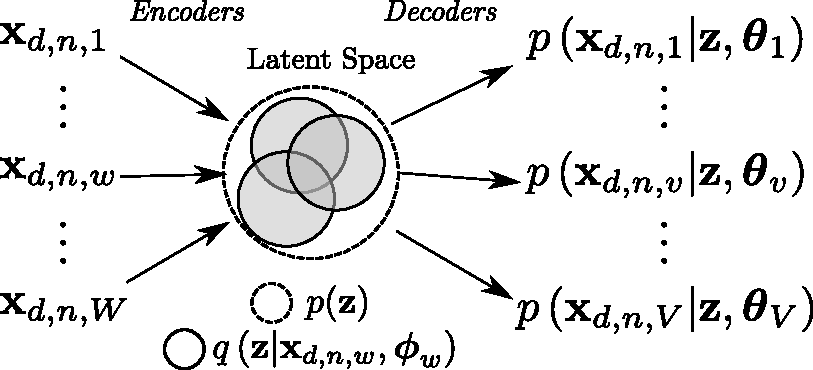
\includegraphics[width=\columnwidth]{./tex/fig/architecture.pdf}
\caption{
General variational framework for our multi-view and multi-dataset model.
Compatibly with the MCVAE formulation, for every pair of views $w$ and $v$
there is a prediction path $w \rightarrow v$ composed by two learnable functions:
the encoding distribution $\q{\z|\xb_w, \phib_w}$ and the decoding likelihood $\p{\xb_v|\z, \thetab_v}$.
Parameters $\phib_w$ and $\thetab_v$ are optimized through \eqnref{eq:argmax} to maximize the likelihood of our generative model under the encoding distributions, and at the same time minimize the Kullback-Leibler distance between every encoding distribution and the prior $\pz$.
}
\label{fig:architecture}
\end{figure}
